\section{Backpropagation and emission synthesis}\label{sec:tool:synthesis}

\subsection{Introduction}
The previous section treated the propagation model of the tool. In order to
simulate the audible sound of aircraft an emission signal is needed. Thus far a
simple signal consisting of noise and a tone was considered. This section
describes a method to create an emission signal from features derived from
recordings. An auralisation or pseudo-recording at a receiver position can then
be created by propagating the signal using the propagation model. Figure
\ref{fig:tool:backpropagation:introduction:block-diagram} shows a block diagram
of the steps that are treated in this section.

\begin{figure}[H]
  \centering
\begin{tikzpicture}[auto, node distance=1cm,>=latex']
\tikzset{
block/.style    = {draw, shape=rectangle, fill=white, minimum height=4em, minimum width=5em, text width=5em, align=center},
}
    % Main nodes
    \node [block]                       (recording)     {Recording};
    \node [block, right=of recording]   (backprop)      {Back-\\propagation};
    \node [block, right=of backprop]    (feature)       {Feature\\extraction};
    \node [block, right=of feature]     (emission)      {Emission\\synthesis};
%     \node [block, right=of emission]    (auralisation)  {Auralisation};

    % Main edges
    \draw [->]  (recording)     --  (backprop);
    \draw [->]  (backprop)      --  (feature);
    \draw [->]  (feature)       --  (emission);
%     \draw [->]  (emission)      --  (immission);

\end{tikzpicture}
  \caption{Block diagram of the backpropagation, synthesis and auralisation method.}
  \label{fig:tool:backpropagation:introduction:block-diagram}
\end{figure}

% An automated procedure was developed to a) backpropagate from source to receiver
% in time-domain and b) analyze the resulting signal to extract features that could be
% used in the development of an emission model or to directly resynthesise the
% emission.

% \subsection{Measurement data}

For the emission synthesis a signal is generated that is based on measurements
that were made for the sonAIR project as described in section
\ref{sec:introduction:sonair}. Figure \ref{fig:figure_trajectory} shows an
overview of the airport, the trajectory and the receiver of the events
considered. Aircraft took off and their height steadily increased from 30 to 260
meters.

% For the data presented measurements from only a single microphone
% were used, situated at a height of 4 meters.


% For the development of the sonAIR model \cite{Zellmann2016} sound recordings
% were made for a large amount of events nearby Z\"{u}rich Airport
% \cite{Zellmann2013}. Along with the sound recordings the position of the
% aircraft was registered and for a subset of the events more detailed information
% was obtained as well, like e.g. thrust settings. Recordings were made at
% multiple positions simultaneously, allowing to determine the directivity of the
% noise components.

\begin{figure}[H]
  \centering
  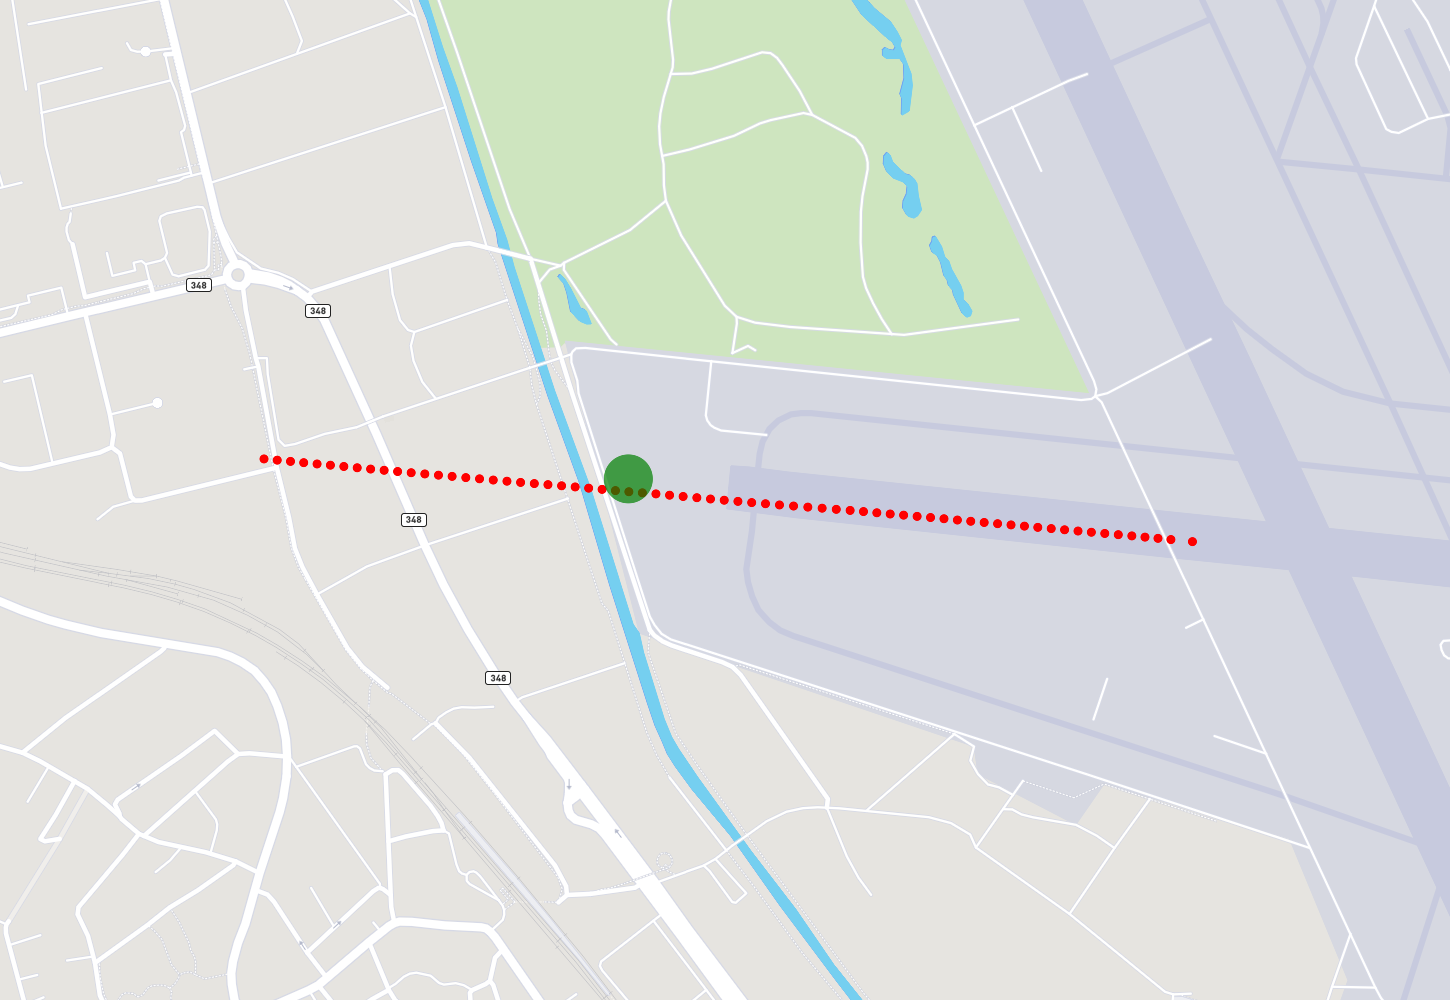
\includegraphics[width=0.3\textwidth]{../figures/manual/auralisation-paper/figure_trajectory}
  \caption{Overview of the airport, trajectory and the receiver. The receiver
(green dot) is situated slightly north of the trajectory, almost straight underneath the
trajectory.}
  \label{fig:figure_trajectory}
\end{figure}


\subsection{Backpropagation}
An automated procedure was developed to backpropagate from receiver to source in
time-domain. The procedure assumes there is only one propagation path,
the direct path, and that the aircraft can be considered a point source.
As shown in Figure \ref{fig:backpropagation_block_diagram}, the
backpropagation algorithm undoes atmospheric attenuation, the Doppler shift, and
geometrical spreading (magnitude) in that specific order, and using the methods as
described in the previous section.
% A recording is taken, and assuming there were no reflections, the atmospheric attenuation and spherical spreading were undone.
Because only the direct path was considered all parameters that were used in the
backpropagation were based on values corresponding to that path.

\begin{figure}[H]
  \centering
\begin{tikzpicture}[auto, node distance=1cm,>=latex']
\tikzset{
block/.style    = {draw, shape=rectangle, fill=white, minimum height=4em, minimum width=5em, text width=5em, align=center},
}
    % Main nodes
    \node [block]                       (immission)     {Immission\\Recording};
    \node [block, right=of immission]   (attenuation)   {Attenuation\\Filter};
    \node [block, right=of attenuation] (delay)         {Spreading\\Delay};
    \node [block, right=of delay]       (spreading)     {Spreading\\Gain};

    % Main edges
    \draw [->]  (immission)     --  (attenuation);
    \draw [->]  (attenuation)   --  (delay);
    \draw [->]  (delay)         --  (spreading);

\end{tikzpicture}
  \caption{Block diagram of the backpropagation model. These steps are applied sequentially to a recording in order to obtain a signal in time-domain that corresponds to the emission of the aircraft.}
  \label{fig:backpropagation_block_diagram}
\end{figure}

Application of the backpropagation algorithm results in a time-domain signal
that corresponds to the emission of the aircraft. The emission includes the
effect of convective amplification, i.e., the directivity effects due to source
motion.

The influence of the ground reflection is non-negligible. A soft ground is still
relatively hard and therefore a -3 dB correction was applied. Ideally, a
microphone on the ground was used, but the dataset that was available consisted
of recordings at a height of 4 meters.

Figures \ref{fig:recording} and \ref{fig:backpropagated} show spectrograms of
respectively the recording and of the signal that was backpropagated. The signal
after backpropagation is shorter than the recording due to lack of aircraft
position information during the initial propagation delay.
Aside from small variations the tonal components remain constant in frequency
over time in Figure \ref{fig:backpropagated}. The variations are caused
by uncertainties in the measured position of the aircraft and thus the estimated
propagation delay.


\begin{figure}[H]
  \centering
  \includegraphics[]{../figures/generated/recording-to-auralisation/recording}
  \caption{
    Spectrogram of a recording of an A320. Clearly visible are the
    Doppler-shifted tones and the peaks due to atmospheric turbulence.
    Interference between direct and reflected path acts as a Comb filter resulting
    in an acoustical Lloyd's mirror-effect, which can be seen here at lower
    frequencies. The most powerful tone corresponds to the blade passing frequency
    of the fan. The other tones are Buzz-Saw tones.}
  \label{fig:recording}
\end{figure}

\begin{figure}[H]
  \centering
  \includegraphics[]{../figures/generated/recording-to-auralisation/reverted}
  \caption{Spectrogram of the recording shown in Figure \ref{fig:recording} after backpropagation to the source. The Doppler-shift has mostly been removed. Artifacts like the mirror-effect and amplitude modulations due to atmospheric turbulence remain.}
  \label{fig:backpropagated}
\end{figure}

\subsection{Feature extraction}
Spectral modelling synthesis was chosen as emission synthesis strategy. With
spectral modelling synthesis a signal is generated as a superposition of tones
and bandpass-filtered noise.
% In order to synthesise the emission of the aircraft
% We're interested in entirely synthesizing the emission of the aircraft and chose to use
% spectral modelling synthesis, that is, a method where a signal is generated
% through a superposition of sines and noise.
Therefore, a method is needed to extract from the backpropagated recordings the
frequency, phase, and level of the tones, as well as the level of the noise as
function of frequency. This section presents a method that was developed for
extracting these features.

The situations considered are landings, and therefore the tonal components in
the spectra are not only the blade passing frequency of the fan and its
harmonics, but also \say{Buzz-Saw} tones. The common denominator of the
frequencies of these components is the frequency at which the engine shaft
rotates.

\subsubsection*{Motivation for method}
The events considered are short, typically less than 30 seconds, and their
spectra vary considerably over time due to directivity of the source. Thus, in
order to get a sufficiently good directivity resolution, a high temporal
resolution is needed, and that limits the possibility to average over time. The
frequency resolution, however, also matters. The emission may contain Buzz-Saw
harmonics with a fundamental frequency below 100 Hz. While that gives some
freedom for using a lower frequency resolution, first the actual tonal
components need to be detected and thus distinguished from the broadband noise.

While already corrected for in the backpropagation, the Doppler shift may make
it difficult connecting obtained frequency-components at one step to those
obtained the step later. Therefore, frequency-tracking algorithms were
considered \cite{Lampert2010}, notably Hidden Markov Models. Due to their
complexity such solutions were not pursued further.

Tone-detection in the frequency-domain is in its simplest form a matter of peak
detection for which a range of algorithms is known. However, a robust algorithm
is needed that can distinguish between the tonal components and broadband noise
peaks.

Initially, the complex cepstrum\footnote{The complex cepstrum is defined as
$c[n] = F^{-1}\left\{\log_{10}{\left( F \left\{x[n]\right\} \right)}\right\}$.}
was used to determine the fundamental frequency of the Buzz-Saw harmonics
(Paper \ref{paper:euronoise2015}). The method was reliable for determining the
fundamental frequency. Because all the tonal components considered are multiples
of this fundamental frequency, all their frequencies would then be known as
well. Unfortunately, the frequency-resolution, or more precisely the
quefrency-resolution, was not high enough to reliably predict the frequency of
the high-frequent components.

\subsubsection*{Tone-seeking algorithm}
Annex C of ISO 1996-2:2007 \cite{ISO1996-2_2007} describes an objective method
for assessing the audibility of tones in noise and a significant part of the
method describes a tone-seeking algorithm. The tone-seeking algorithm works in
frequency-domain on a narrowband power spectrum. An estimate of the narrowband
spectrum is obtained using Welch's method. The time signal is split in chunks, a
Hanning window is applied to each chunk, and a periodogram is determined for
each chunk. Finally, linear averaging over the chunks results in Welch's
estimate of the power spectral density.

According to the standard an A-weighted signal should be used. Because the
frequencies of the tonal components are of interest, and not their audibilities,
an unweighted signal is considered instead. Furthermore, in order to obtain an
accurate estimation an averaging-time of one minute is required, however, this
could not be done as explained.

The tone-seeking algorithm first determines noise pauses, which are local maxima
with a probability of a tone. The next step is to assess whether tones exist in
these noise pauses. Each frequency bin or line is assigned a label indicating whether
it is part of a tone or whether it is masking noise.
% The tone-seeking algorithm was implemented according to the standard.

The power of the lines that are part of a tone are integrated. A correction is
made for the masking noise contributions to those lines by estimating their
contribution from a regression through the lines marked as noise within a
portion of the critical band\footnote{A critical band is the bandwidth of a
filter created by the cochlea, the auditory part of the inner ear.} around the
centerfrequency of the tone.

\subsubsection*{Extension}
The tone-seeking algorithm is capable of detecting many of the tonal components
but not all of them. Because the tones of interest are all multiples of a
fundamental frequency the goal is to determine this fundamental frequency
sufficiently accurate. The assumption was therefore made that all tones found by the
tone-seeking algorithm from the standard were harmonics and that the fundamental
frequency was within a specified range.
The fundamental frequency is then given
\begin{equation}
 f_{0} = \mathrm{gcd}\left(f_1, f_2, \dots, f_n \right)
\end{equation}
where $\mathrm{gcd}$ is the \emph{greatest common divisor} (Paper \ref{paper:internoise2016}).
Implementations of the $\mathrm{gcd}$ operator attempt to find an exact solution.
Due to errors in the estimation of the frequency of the tones and because some tones are
not harmonics, an exact solution does not exist. Given an initial estimate of
the fundamental frequency, one could define an error as the sum of the squared
deviation between the target order of the harmonics and the actual estimated
order
\begin{equation}
 e = \sum_{i=0}^{n} \left( \frac{f_i}{f_0} - \mathrm{round}\left(\frac{f_i}{f_0}\right) \right)^2
\end{equation}
An estimate of the fundamental frequency is obtained by minimising this error.

The tone-seeking algorithm is first ran to detect tonal components and obtain their centerfrequencies.
% TODO bandwidth!
Then, a fundamental frequency estimation is done. Next, the frequency lines
within ??? hertz are added as noise pauses.
The tone-seeking algorithm determines for these lines again whether they could
be tones and outputs levels for all tonal components.
Finally, the masking noise lines were integrated in \nicefrac{1}{6}-octaves.


% An earlier version of the algorithm did not use the $\mathrm{gcd}$ in
% combination with the optimisation algorithm but instead determined the
% fundamental frequency using the complex cepstrum (Paper ).
% While it was possible to reliably determine the fundamental frequency with the
% complex cepstrum, the value which was obtained was not sufficiently accurate
% for determining higher harmonics.

% In the method as described in Annex C of ISO 1996-2:2007 each spectral line is
% assigned a label, e.g. whether the line is part of a tone or noise. Tones
% typically have a bandwidth and can therefore, depending on the frequency
% resolution, be spread over multiple lines. In order to compute the level of a
% tone, the spectral lines corresponding to that tone need to be integrated.

The bandwidth of the tonal components depends on various aspects, like frequency
or phase modulations at the source or during propagation, e.g. due to
atmospheric turbulence. The direct and reflected contribution are
Doppler-shifted slightly differently and that causes either double peaks or a
single broader peak. But also averaging time and window shape play a role.

% The center frequencies of the tonal components obtained with the enhanced method
% were fed back in the method of the standard to obtain labels for each spectral
% line and to compute the levels of the tones and the noise.

% The lines that were assigned noise were integrated into \nicefrac{1}{6} octaves and for each
% fractional octave its level was kept.

For the feature extraction two seconds windows were used, without overlap.
While a short window decreases frequency resolution and precision of the
features, a short
window was required in order to provide temporal resolution of the features.
A 2 seconds window proved to be a good balance between temporal resolution
and frequency resolution. A value for the phase could not be obtained because
the signal was too noisy.

% For the development of an emission model it is expected that
% the uncertainties could be reduced through ensemble averaging. % TODO include this?

\subsection{Emission and immission synthesis}\label{sec:tool:synthesis:synthesis}
% As mentioned before the emission was synthesised using spectral modelling
% synthesis.
With the extracted features, which were obtained as function of time and at
several receiver positions, it is possible to develop an emission model that
takes into account directivity of the spectral components. Such emission model
would then output input for the SMS synthesiser and the created emission signal
would be propagated to a receiver a location.

An important question to ask is whether the described methodology of extracting
features, synthesising an emission signal and propagating it would result in
plausible auralisations. For example, it could be possible that the chosen
synthesis strategy and features cannot reproduce certain characteristics in the
sound. Therefore, the next chapter describes a comparison between auralisations
and recordings with the auralisations based on recordings.

For a specific event and receiver, the immission was backpropagated and features
were extracted. These features were used to re-synthesise the emission. The
emission signal was propagated to the receiver, and a direct path and a single
reflection were considered. The assumption was made that the emission is
identical for the emission angles corresponding to direct and reflected path.

The feature extraction method provided frequencies and levels of tonal
components as function of time. Variations in the frequencies as function of
time could be observed, but with a two second window that would result in only
few data points. Variations in frequency were therefore ignored and computed was an
average value for the fundamental and each of the harmonics.

As mentioned in the previous section, values for the phase of the tones could
not be obtained, and therefore values had to be chosen. Because the harmonics
are \say{Buzz-Saw} noise, a phase corresponding to a sawtooth signal was
initially assumed. Participants in a preliminary test found the simulations
sound metallic compared to the recordings (Paper \ref{paper:internoise2016}). Therefore, the
assumption was made that the initial phase relation between the Buzz-Saw tones
was entirely lost and could therefore be chosen randomly. In that case the
probability distribution would be uniform.

Figures \ref{fig:synthesis} and \ref{fig:auralisation} show spectrograms of
respectively the emission synthesis and the auralisation at the receiver.

\newpage
\afterpage{
\begin{figure}[H]
  \centering
  \includegraphics[]{../figures/generated/recording-to-auralisation/synthesis}
  \caption{Emission synthesis of the aircraft. Inputs to the emission synthesiser were obtained by applying the feature-extraction algorithm to the signal shown in Figure \ref{fig:backpropagated}. The level of the tonal components vary over time. The blade passing frequency is not clearly visible because the determined level of the tone was underestimated.}
  \label{fig:synthesis}
\end{figure}


\begin{figure}[H]
  \centering
  \includegraphics[]{../figures/generated/recording-to-auralisation/auralisation}
  \caption{Auralisation of the event shown in Figure \ref{fig:recording} .
  The Doppler-shifted tones and the mirror-effect are clearly visible. The Doppler-shifted tones are not very smooth. This is due to fluctuations in the aircraft position due to uncertainties.}
  \label{fig:auralisation}
\end{figure}
}


%
%
%
%
%
%
%
%  TODO: BELOW IS OLD STUFF
%
%
% \section{Emission model}
%
% The emission model describes the emission of aircraft. In this section we discuss the development of the model as well as the eventual implementation.
%
% As described in \ref{sec:theory_aircraft_emission_models} several emission models exist.
%
% What is needed for the auralizations is a model that can describe tonal and noise components.
% The models referred to all predict sound levels in fractional-octaves.
%
% Therefore, we will now try to extract the relevant features using an automated method. The method is roughly as follows:
%
% \begin{enumerate}
%  \item Backpropagate from source to receiver in time-domain, undoing the Doppler shift, atmospheric attenuation and spreading. The ground effect is ignored for now. We now have a signal that roughly corresponds to what is emitted from the airplane.
%  \item Determine fundamental frequency. An aircraft spectrum consists mostly of noise and tones, which are mostly harmonics. Knowing the fundamental frequency, allows you to determine the power of not only the fundamental, but also of each harmonic.
%  \item And that is the final step. Determine power of the tones, and consider the rest of the spectrum as noise.
% \end{enumerate}
%
%
%
% \subsection{Empirical model}
% In the sonAir project aircraft landings and take-offs were recorded.
%
% \subsubsection{sonAir data acquisition}
%
% \newpage
% \section{Backpropagation in time-domain}
% To backpropagate in time-domain an inverse propagation model was developed that is based on the propagation model explained in \ref{}.
% The inverse propagation model undoes the intensity loss due to geometrical spreading, as well as the propagation delay that causes the Doppler shift.
% Furthermore, the inverse propagation model corrects for atmospheric attenuation.
% One effect the inverse propagation model cannot undo is the ground effect.
%
%
% \subsubsection{Limitations of the method}
%
%
% \subsubsection{Ground effect}
%
%
%
%
% Now that some of the propagation effects have been undone we have a signal that roughly corresponds to as if you would fly along with the aircraft, and rotate around it.
%
%
% \missingfigure{Spectrum of the recorded signal after backpropagating in time-domain.}
%
% \missingfigure{Power spectrum of the reverted signal.}
%
% \newpage
% \subsection{Determine fundamental frequency}
% To determine the fundamental frequency in an automated and reliable way, several methods were tried.
%
% \subsubsection{Using complex cepstrum}
%
% Using the complex cepstrum it was possible to obtain an accurate estimate for the fundamental frequency. However, the estimate proved not accurate enough to determine the higher-frequency harmonics.
% Since the frequency of an harmonic is the fundamental multiplied by the order, any inaccuracy in the estimate is multiplied as well. For harmonics around the blade passing frequency and up the error was generally too big.
% Therefore, another method was sought.
%
% \missingfigure{In the complex cepstrum a peak can be found that corresponds to the fundamental frequency.}
%
% \subsubsection{Estimate fundamental from determined tones}
% Estimating the fundamental frequency directly from a spectrum result in an inaccurate estimate. However, when using multiple harmonics, and especially higher order harmonics, the estimate in the error can drop significantly.
%
% \begin{enumerate}
%  \item Determine frequency of harmonics using a tone-seeking algorithm.
%  \item Estimate fundamental frequency given the frequencies of the harmonics.
% \end{enumerate}
%
% An example of a simple tone-seeking algorithm is one that checks when, in the estimate of the power spectrum, the steepness gets above or below a certain threshold. When the threshold is passed twiced - the second sweep in opposite direction - a tone might be present.
% ISO 1996-2:2007 Annex C provides an objective method for assessing the audibility of tones in noise, and part of the method is a tone-seeking algorithm that does exactly this. Aside from the tone-seeking algorithm, the objective method also provides a method for assessing the tones, including estimating their power.
%
% \fbox{\begin{minipage}{0.5\textwidth}
% A method to verify whether audible tones are present in a signal is provided in ISO 1996-2:2007 Annex C. Based on the prominence of tones, the method also provides recommended level adjustments.
% \begin{enumerate}
% \item Find preliminary noise pauses.
% \item Search for tones in noise pauses.
% \item Put a critical band on the centerfrequency of the tone, and determine the tone strength, masking noise level and finally the tonal audibility.
% \item The final tonality adjustment is determined by the tone with the highest tonal audibility.
% \end{enumerate}
% \end{minipage}}
%
% \missingfigure{Tones and critical bands assessed using an implementation of ISO 1996-2:2007 Annex C}
%
% Using a tone-seeking algorithm like the one provided by the standard, one can obtain estimates of the frequencies of tonal components. However, it is not yet known which harmonic order the tone has, or in fact whether it is a harmonic at all.
% Even so, assuming the tones are all harmonic and exact, then the fundamental frequency $f_{0}$ would be the greatest common divisor of the harmonics $f_i$
% \begin{equation}
%  f_{0} = \mathrm{gcd}\left(f_1, f_2, \dots, f_n \right)
% \end{equation}
% Implementations of the $\mathrm{gcd}$ attempt to find an exact solution. However, due to errors in the estimate of the tones (because of a limited frequency resolution) and because some tones are not harmonics, an exact solution would not exist.
% Given an initial estimate of the fundamental frequency, one could define an error as the sum of the squared deviation between the target order of the harmonics and the actual (inaccurate) order
% \begin{equation}
%  e = \sum_{i=0}^{n} \left( \frac{f_i}{f_0} - \mathrm{round}\left(\frac{f_i}{f_0}\right) \right)^2
% \end{equation}
% The fundamental frequency is obtained by minimizing this error. Without constraining the fundamental frequency, incorrect estimates are likely to be obtained. For example, an estimate of the fundamental that is half the actual frequency would fit. And a lower frequency, would also result in a smaller error, causing a preference for a very low-frequency fundamental.
% In our case, we know that the fundamental frequency is generally between 60 and 80 Hz, eliminating both problems.
%
% However, it might still happen that several tones are estimated to be the same harmonic - which is obviously incorrect - and thereby increasing the error in the estimate of the fundamental.
% This can be prevented by checking all combinations with each combination consisting of only unique harmonics. The combination that minimises the error is kept.
%
% The eventual method is:
% \begin{enumerate}
%  \item Estimate frequencies of tones using the tone-seeking algorithm described in ISO 1996-2:2007 Annex C.
%  \item Estimate which harmonic order the tones are.
%  \item Obtain initial estimate of fundamental frequency from the estimated tone frequencies and harmonic orders using a least-squared method. An error is defined as the sum of the absolute deviation between frequency estimate given by 1, and the harmonic order multiplied with the fundamental frequency.
%  \item It might occur that multiple tones would seem to correspond to the same harmonic. This is not possible and should be prevented.
%  \item Therefore all combinations of harmonic order estimates are checked. The result with the smallest error is the final result of the algorithm.
% \end{enumerate}
%
% \newpage
% \subsection{Determine features}
% With the estimate of the fundamental frequency, we also know what the frequencies
% of the harmonics are. The ISO method not only provides an algorithm to determine
% tones, but also a method for assessing them.
%
% We now feed the estimated harmonics back into the ISO method, setting noise
% pause starts and ends at $f_i -/+ f_c/8$. The tone level and bandwidth is is
% determined for each tone, overriding the requirements that frequency lines
% within 6 dB of the maximum should be present, and that the bandwidth should be
% less than 10\% of the critical band.
%
% The frequency of each of these tones is kept as well. The noise lines are
% integrated per fractional-octave.
%
% \begin{table}[h]\centering
%   \caption{Overview of the features.}
%     \begin{tabular}{ | l | l | l | p{5cm} |}
%     \hline
%     Component & Feature & Time-variant \\ \hline
%     Tone & center frequency & yes \\ \hline
%     Tone & bandwidth & yes \\ \hline
%     Tone & sound pressure level & yes \\ \hline
%     Noise & fractional-octave center frequency & no  \\ \hline
%     Noise & fractional-octave band designator & no  \\ \hline
%     \end{tabular}
% \end{table}
%
% \subsubsection{Noise floor}
% The signal-to-noise ratio is dependent on range and thus time. For the samples that were analysed, the noise floor took over at between 8 and 12 kHz.
% For this reason features were only extracted below 8 kHz.
%
% % Knowing the bandpass
% % Furthermore, ISO 1996:2-2007 describes for each frequency line whether it is consider a tone, noise, or neither.
% % This signal can be used to extract relevant features.
% % Many methods exist to detect and track tonal components.
% % ISO 1996-2:2007 Annex C provides an objective method for assessing the audibility of tones in noise.
%
%
% \newpage
% \subsection{Verify features through an auralization}
% Before analysing the features and developing an emission model from them, its important to ask
% the following question. Are these features sufficient to create a realistic
% emission signal? Or, even better, are these features, taking into account the
% developed propagation model, providing a realistic signal at the receiver? Does,
% what you hear, really sound like an aircraft? That is after all the aim.
%
% To verify whether the features contain enough information in order to create a
% plausible auralization, an emission signal was constructed from the features,
% and propagated to the receiver that was used for the measurement.
%
% \subsubsection{Synthesis of emission signal}
% The features that were obtained every second were linearly interpolated to a sample frequency of 22 kHz and were smoothed by applying a rolling mean in both directions.
% The only exception were the frequencies of the harmonics, for which average values were taken. % EXPLAIN!!
% The components are added together resulting in the final signal.
% Figure \ref{} shows a spectrogram of a synthesized emission signal.
%
% \missingfigure{Spectrogram of synthesized emission signal}
%
% \missingfigure{Unweighted sound pressure level as function of time. Fast time-weighting was applied.}
%
% \newpage
% \subsubsection{Signal at receiver}
% We now try to model the propagation of the original event as accurate as
% possible. A virtual receiver is positioned where the real receiver was. Below
% the receiver a flat ground is modelled, disregarding small height differences
% that are present in reality. The ground is modelled to be grass entirely, with
% the impedance calculated using ........
%
% A moving point source follows the original trajectory. The synthesized emission
% signal is now fed directly into the propagation model and is used for both the
% direct path as well as possible reflected paths. The virtual source is modelled
% as a omni-directional source because the synthesis already includes the gain
% adjustment due to source directivity. However, this gain is for a fixed set of
% angles i.e., the angles corresponding to the direct path. For the reflected
% paths the directivity would in reality be slightly different but this effect
% cannot be included in this verification.
%
% Included propagation effects were....
%
% Figure \ref{} shows a spectrogram of a verification auralization as well as a spectrogram of the original recording and figure \ref{} shows the A-weighted sound pressure level as function of time for both.
% \missingfigure{Spectrogram of synthesized emission signal and recording.}
% \missingfigure{A-weighted sound pressure level as function of time. Fast time-weighting was applied.}
%
%
% \newpage
% \subsection{Model}
%



